\chapter[Environmental Variables]{Environmental Variables in Species Distribution Modeling}

\begin{objetivos}
By the end of this chapter, readers should understand the role of environmental
variables in SDM; distinguish climatic, topographic, edaphic, and derived
predictors; identify resources such as WorldClim, CHELSA, EarthEnv, SoilGrids,
and ENVIREM; understand spatial resolution, geographic extent, coordinate
reference systems (CRS), resampling, cropping, and layer harmonization; build
reproducible environmental stacks in R; and apply these concepts to
\textit{Dinizia excelsa} across the Amazon biome.
\end{objetivos}

\section{Environmental Variables in SDM}

Environmental variables provide the explanatory basis of species distribution
models. They represent climatic, edaphic, topographic, hydrological, or
structural gradients used to characterize occurrence locations and the sites
available for model calibration and projection. The ecological quality of an
SDM therefore depends on the coherence among the occurrences, calibration area,
spatial scale, and selected predictors
\parencite{guisan2005predicting,elith2009,guisan2017habitat}.

In correlative models, environmental variables serve as predictors of
statistical occurrence--environment relationships. These associations should
not automatically be interpreted as causal. A variable may directly represent
an ecological process, but it may also act as a proxy for an unmeasured gradient
\parencite{franklin2010,guisan2017habitat}.

\begin{conceito}[title={\faBook\quad An environmental variable is not necessarily an ecological mechanism}]
A variable represents a gradient associated with species distribution. High
statistical importance does not establish direct causality. Ecological
interpretation must consider natural history, spatial scale, data resolution,
the candidate predictor set, and prior knowledge of limiting processes.
\end{conceito}

\subsection{Environmental Space, Resolution, and Scale}

Environmental space is the set of conditions represented by model predictors.
Whereas geographic space consists of coordinates, pixels, polygons, and maps,
environmental space consists of the variable values associated with each
location. Distant sites may be environmentally similar, while nearby sites may
differ sharply along gradients of elevation, soil, moisture, or vegetation.

Spatial resolution defines the smallest analytical unit---the pixel size in a
raster. Geographic extent defines the total area considered. Ecological scale
simultaneously involves resolution, extent, time, and level of biological
organization. Climate often dominates at broad scales, whereas soil,
topography, hydrology, land cover, and microclimate may be decisive regionally
or locally.

\begin{atencao}[title={\faExclamationTriangle\quad Compatibility between occurrences and environment}]
Environmental-layer resolution must be compatible with occurrence precision.
A record with several kilometers of spatial uncertainty should not be treated
as a precise observation within a raster cell only a few meters wide.
\end{atencao}

\section{WorldClim}

WorldClim is among the most widely used climatic databases in SDM. It provides
global temperature, precipitation, and derived bioclimatic layers at several
resolutions. BIOCLIM variables summarize mean, extreme, and seasonal aspects of
climate and are widely used in ecological-niche, biogeographic, and climate
change studies \parencite{fick2017worldclim}.

\begin{conceito}[title={\faBook\quad BIOCLIM variables}]
BIOCLIM variables are climatic descriptors derived from monthly temperature and
precipitation. They include annual means, thermal seasonality, temperatures of
the warmest and coldest quarters, annual precipitation, precipitation
seasonality, and precipitation of the wettest, driest, warmest, and coldest
quarters.
\end{conceito}

\section{CHELSA}

CHELSA is a high-resolution global climate database designed to represent
climatic patterns while accounting for orographic and atmospheric processes.
In mountainous or topographically heterogeneous regions, it may represent
temperature and precipitation gradients better than simpler interpolation
products \parencite{karger2017chelsa}.

\begin{dica}[title={\faLightbulb\quad WorldClim or CHELSA?}]
WorldClim is widely used and readily accessible. CHELSA may be particularly
valuable in mountainous areas, regions with strong topographic variation, or
studies sensitive to orographic precipitation. The choice should reflect the
region, scale, objective, and consistency with future projections.
\end{dica}

\section{EarthEnv}

EarthEnv brings together global products for characterizing environmental
heterogeneity, including variables derived from topography, climate, land
cover, and habitat. In SDM, heterogeneity metrics can support analyses of
endemism, beta diversity, environmental refugia, and habitat differentiation
\parencite{amatulli2018data}.

\section{ENVIREM}

ENVIREM extends the conventional bioclimatic set with indices having stronger
ecophysiological interpretations, including potential evapotranspiration,
climatic moisture, continentality, and water--energy balance. These variables
may improve environmental representation in ecological-niche models
\parencite{title2018envirem}.

\section{Topographic Variables}

Variables derived from digital elevation models can represent important SDM
gradients. Elevation, slope, aspect, roughness, topographic position, and terrain
heterogeneity influence microclimate, drainage, solar exposure, erosion, water
accumulation, and habitat distribution \parencite{farr2007srtm}.

Although Amazonia is less topographically variable than major mountain systems,
topography can still represent gradients related to drainage, relative
elevation, terra firme forest, floodplains, escarpments, interfluves, and local
hydrological conditions.

\section{Edaphic Variables and SoilGrids}

Edaphic variables represent environmental filters related to fertility,
texture, acidity, cation-exchange capacity, water retention, and nutrient
availability. SoilGrids, developed by ISRIC, provides global predictions of
soil properties at multiple depths for regional and global SDM applications
\parencite{poggio2021soilgrids}.

\begin{conceito}[title={\faBook\quad Soil as an ecological filter}]
Soil is a comparatively stable landscape component and may explain
distribution patterns not captured by climate alone. For plants, pH, texture,
organic carbon, clay, sand, and cation-exchange capacity may be strongly
associated with occurrence.
\end{conceito}

\section{Harmonizing Environmental Layers}

Environmental databases often differ in resolution, extent, coordinate system,
and units. Layers must therefore be harmonized before use. The process includes
cropping, reprojection, resampling, standardized naming, removal of redundant
layers, and construction of a consistent environmental stack.

\begin{atencao}[title={\faExclamationTriangle\quad Harmonize before modeling}]
Never combine environmental rasters with different resolutions, extents, or
projections without harmonization. Spatial inconsistencies can produce
incorrect extractions and compromise the entire model.
\end{atencao}

\section{Case Study: Environmental Variables for \textit{Dinizia excelsa}}

The preceding concepts are now applied to \textit{Dinizia excelsa} in the
Amazon biome. Its occurrences were compiled, cleaned, spatially filtered, and
thinned in Chapter 2. They are now linked to real environmental layers cropped
and harmonized to the biome extent.

The goal is not simply to generate environmental maps, but to prepare a
spatially coherent foundation for multicollinearity control, variable selection,
model fitting and evaluation, ensembles, future climate projections, and
paleoclimatic reconstructions.

\begin{aplicacao}
The environmental variables are treated as ecological hypotheses about the
gradients that may influence \textit{Dinizia excelsa}. Climatic predictors
represent energy and water filters; topographic predictors represent terrain
heterogeneity; and edaphic predictors, when available, represent substrate and
fertility filters.
\end{aplicacao}

\subsection{Selected Bioclimatic Variables}

WorldClim bioclimatic variables were prepared and cropped to the Amazon biome.
The selected predictors represent temperature, precipitation, and seasonality:

\begin{itemize}
  \item BIO3 -- Isothermality;
  \item BIO4 -- Temperature seasonality;
  \item BIO5 -- Maximum temperature of the warmest month;
  \item BIO8 -- Mean temperature of the wettest quarter;
  \item BIO12 -- Annual precipitation;
  \item BIO13 -- Precipitation of the wettest month;
  \item BIO14 -- Precipitation of the driest month;
  \item BIO18 -- Precipitation of the warmest quarter; and
  \item BIO19 -- Precipitation of the coldest quarter.
\end{itemize}

These variables represent climatic components related to water availability,
thermal stress, seasonality, and environmental extremes. For tropical trees,
such gradients may affect survival, growth, regeneration, recruitment, and
population persistence.

\rscriptfile{scripts/unidade03/01_variaveis_ambientais_dinizia.R}

\begin{figure}[H]
  \centering
  \includegraphics[width=0.98\textwidth]{figuras/unidade03/unidade03_variaveis_bioclimaticas_dinizia.png}
  \caption{Selected bioclimatic variables for the Amazon biome and final occurrence records of \textit{Dinizia excelsa}. Each panel has an independent color scale to display gradients of temperature, precipitation, and seasonality.}
  \label{fig:unidade03_variaveis_bioclimaticas_dinizia}
\end{figure}

\subsection{Topographic Variables}

The script also derives topographic variables from a digital elevation model:
elevation, slope, and aspect. These layers are harmonized with the bioclimatic
variables to ensure identical resolution, extent, spatial mask, and CRS.

\begin{figure}[H]
  \centering
  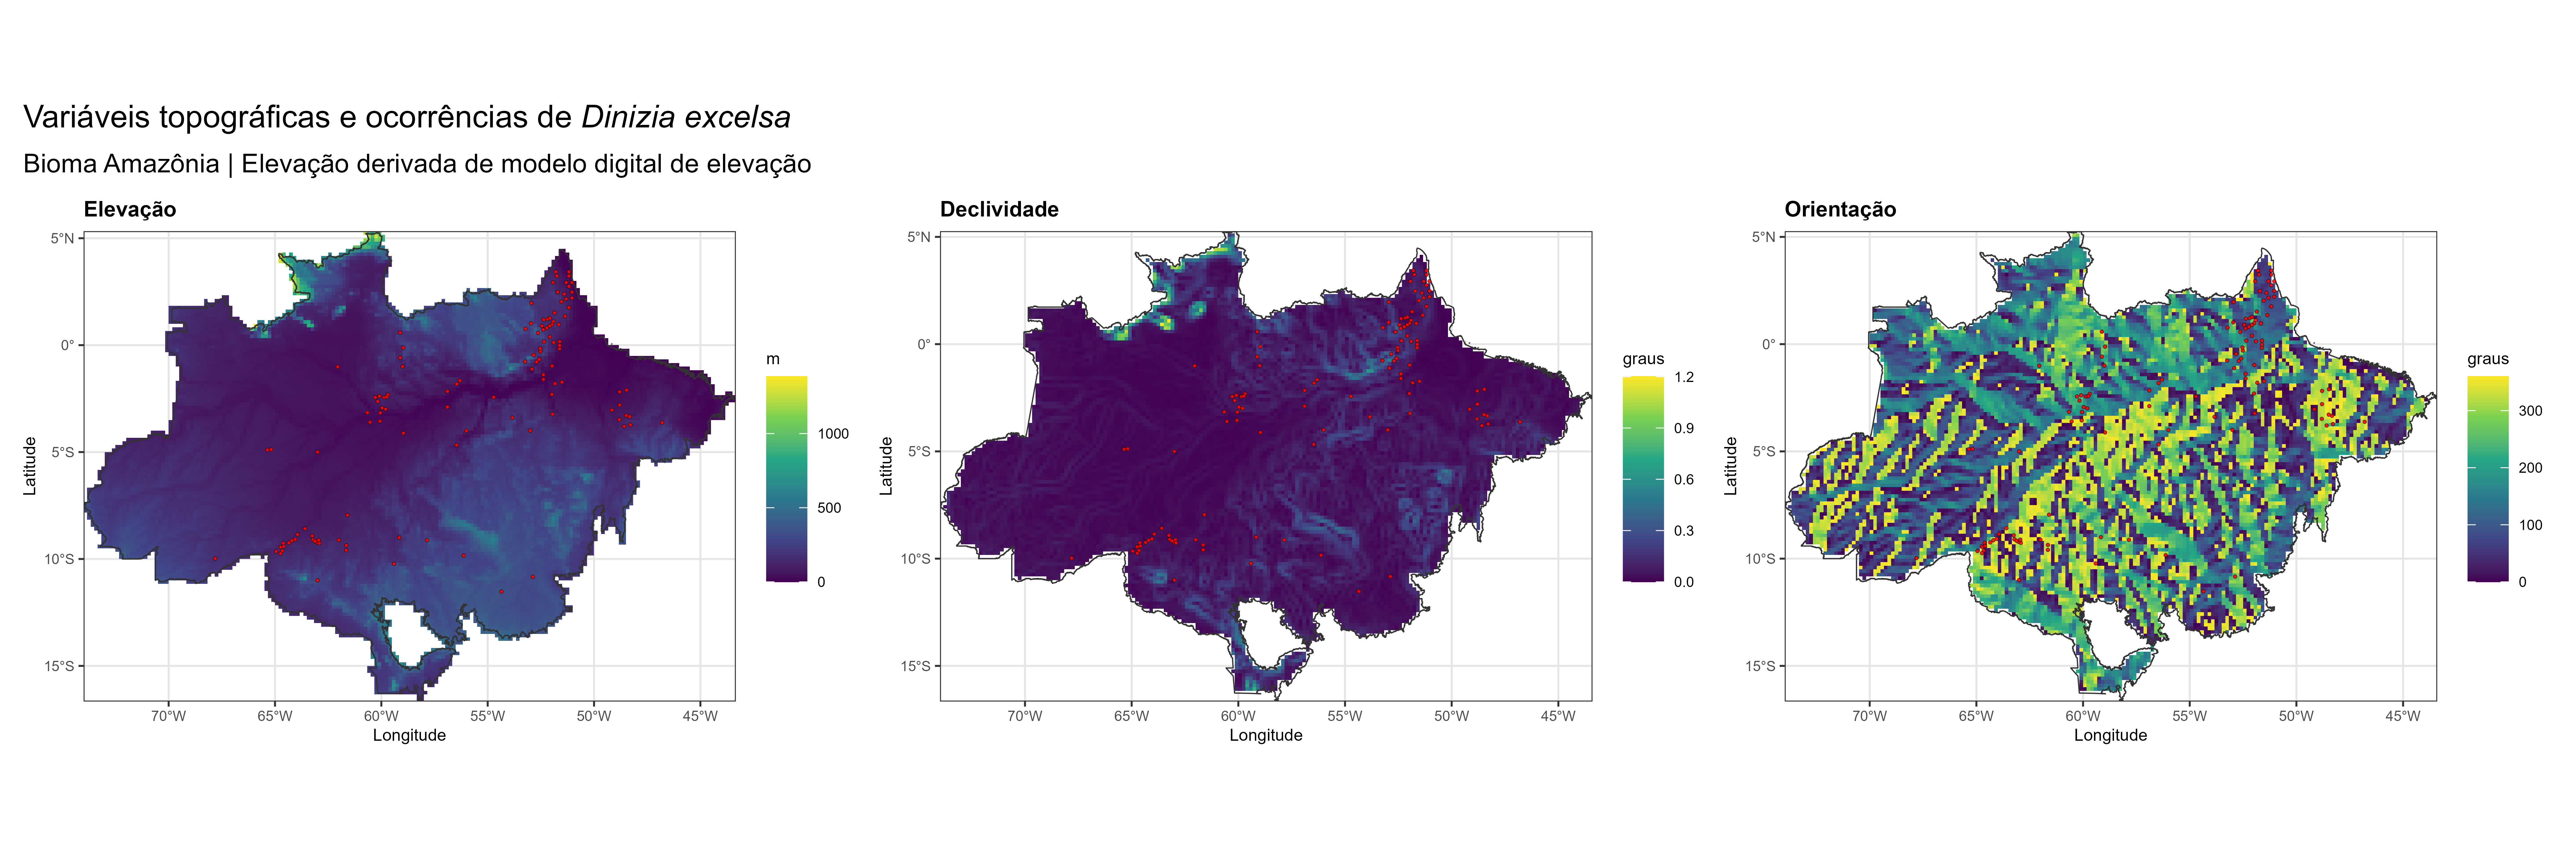
\includegraphics[width=0.98\textwidth]{figuras/unidade03/unidade03_variaveis_topograficas_dinizia.png}
  \caption{Topographic variables prepared for the Amazon biome and the \textit{Dinizia excelsa} case study: elevation, slope, and aspect.}
  \label{fig:unidade03_topografia_dinizia}
\end{figure}

\subsection{Environmental Extraction at Occurrence Locations}

After layer preparation, the value of every predictor is extracted at each
final occurrence location. This environmental matrix characterizes the
species' occupied range, supports correlation analysis and predictor selection,
and provides input for suitability models.

\begin{figure}[H]
  \centering
  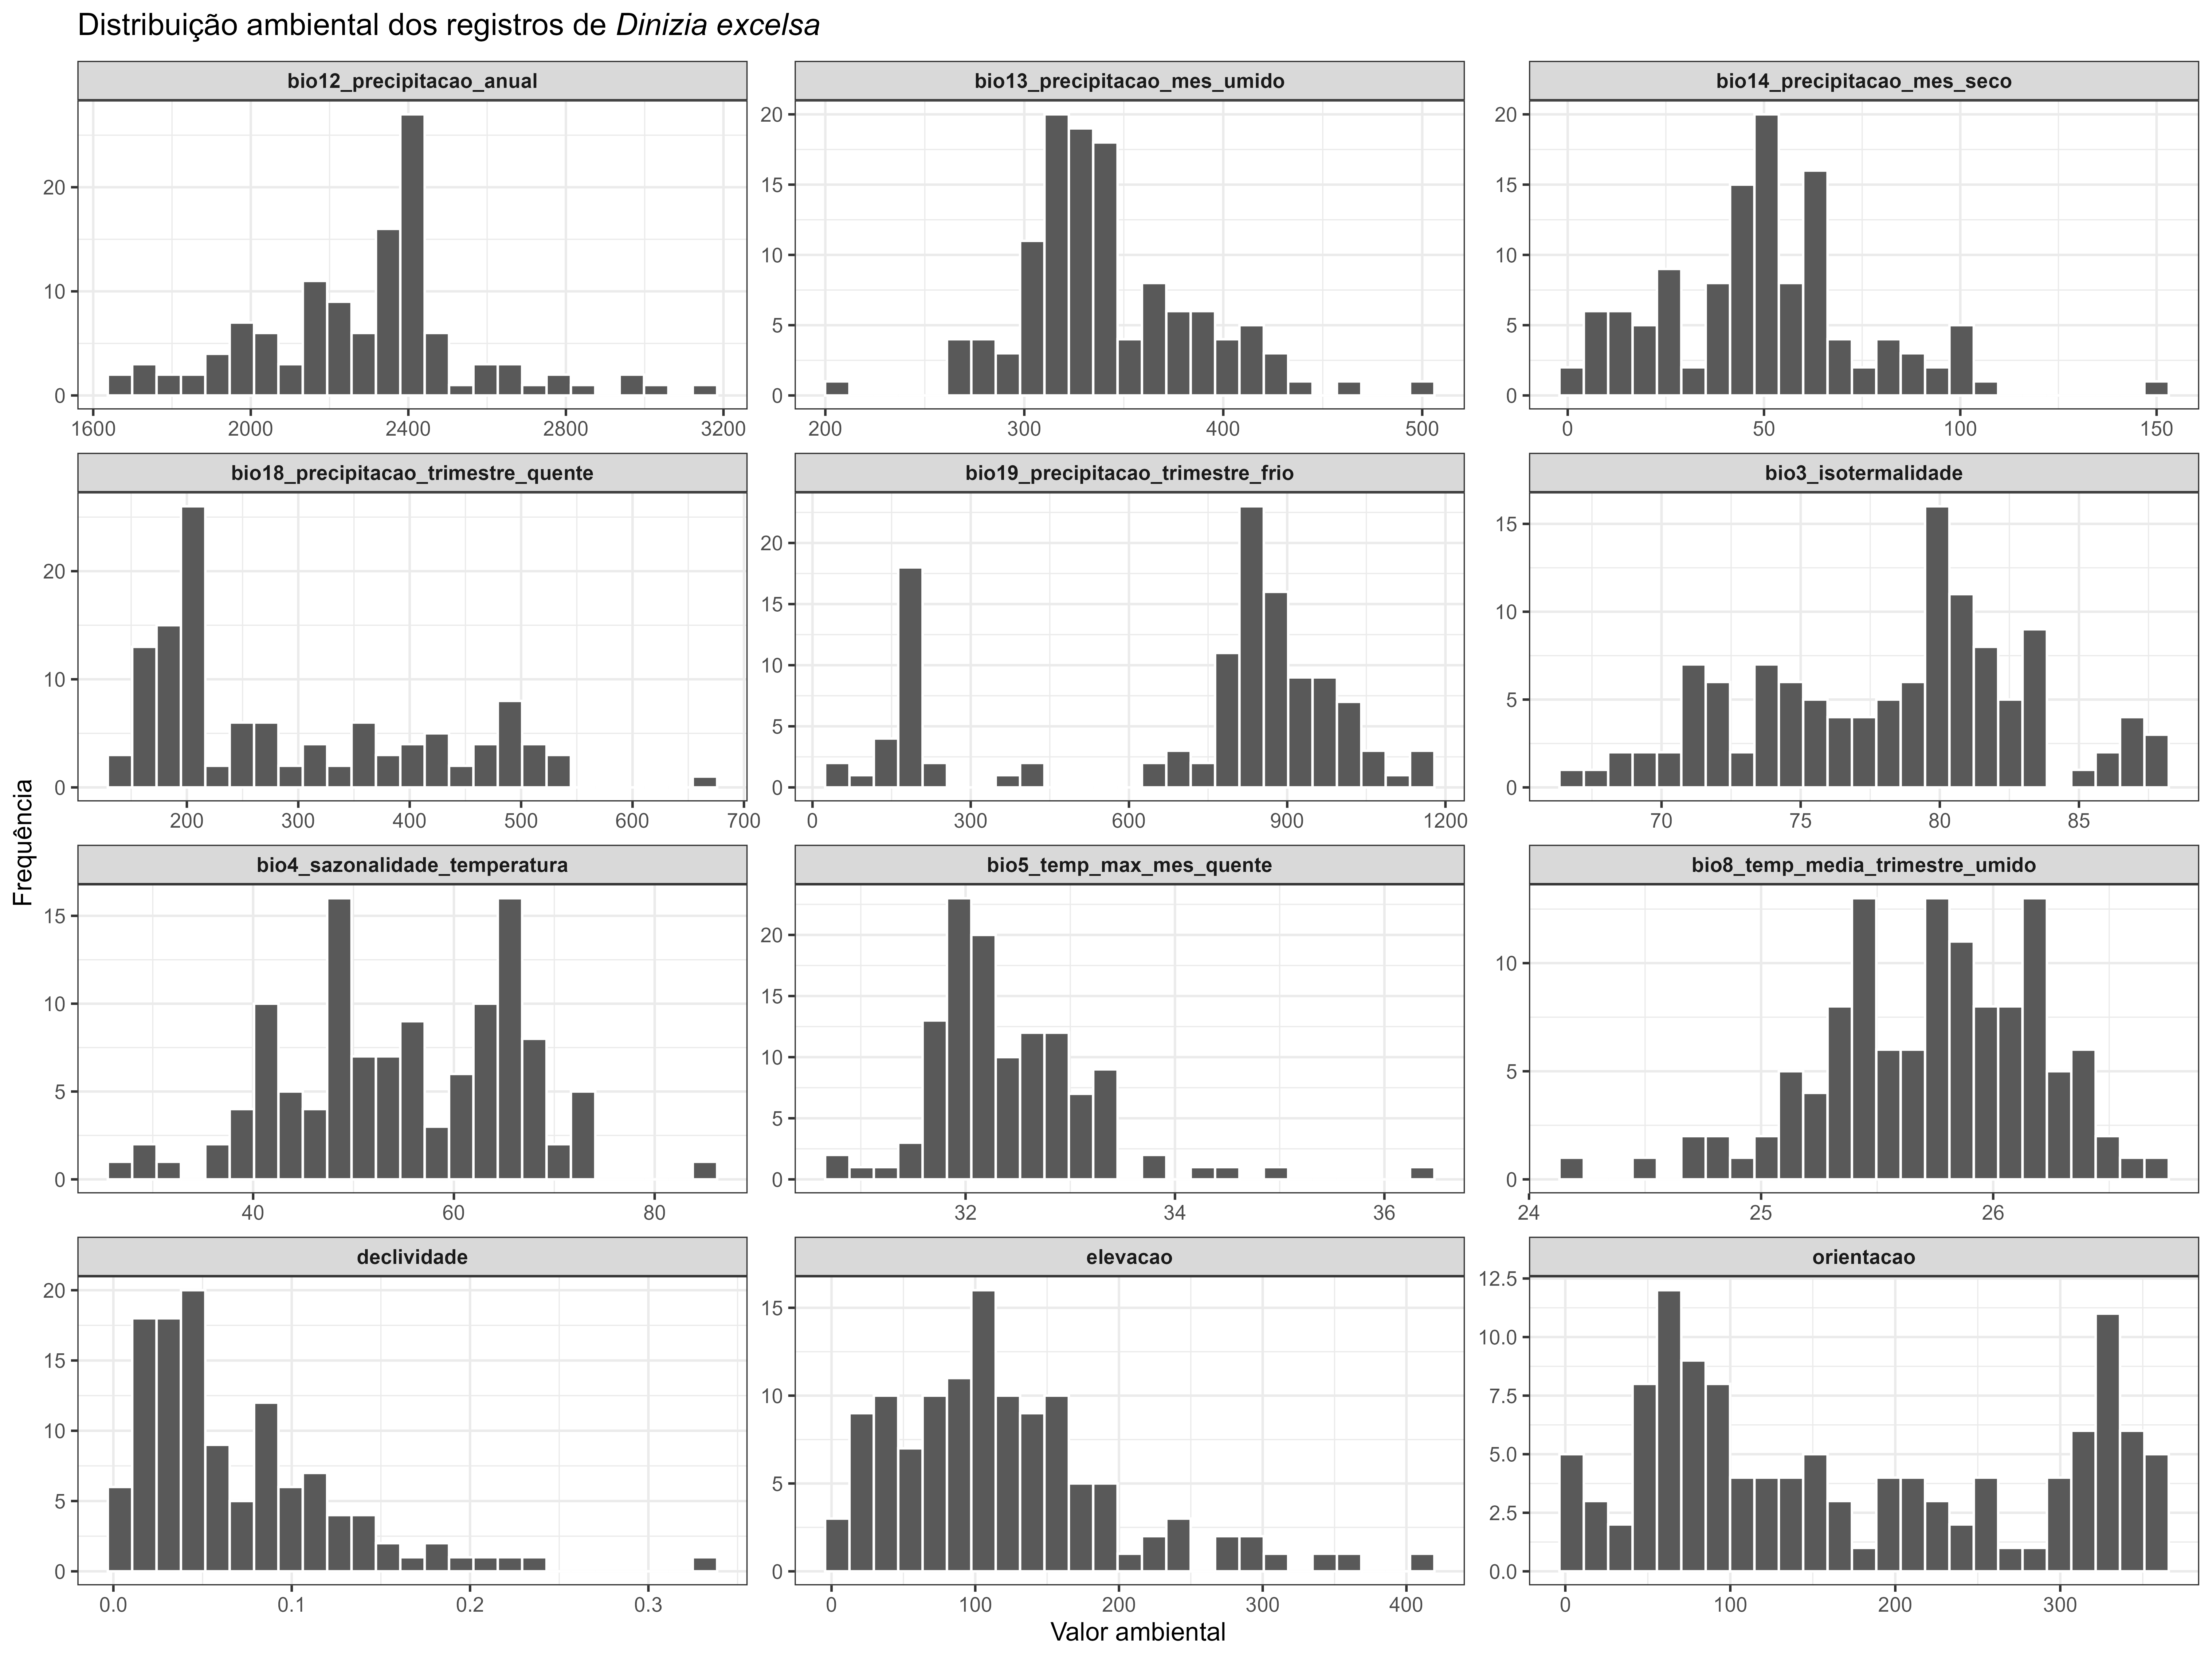
\includegraphics[width=0.94\textwidth]{figuras/unidade03/unidade03_histogramas_ambientais_dinizia.png}
  \caption{Distributions of environmental variables extracted at final \textit{Dinizia excelsa} occurrences. The histograms characterize the environmental range occupied by the species.}
  \label{fig:unidade03_histogramas_dinizia}
\end{figure}

\section{Outputs from Chapter 3}

The chapter script produces:

\begin{itemize}
  \item a multivariate raster of selected bioclimatic variables for Amazonia;
  \item a raster of harmonized topographic variables;
  \item the complete environmental stack used in later chapters;
  \item a table of environmental values at \textit{Dinizia excelsa} occurrences;
  \item an environmental background sample for the Amazon biome;
  \item environmental-layer metadata; and
  \item bioclimatic maps, topographic maps, and environmental histograms.
\end{itemize}

\begin{dica}[title={\faLightbulb\quad File organization}]
Retain these outputs for subsequent chapters. The stack saved as
\texttt{dados/unidade03/processados/variaveis\_ambientais\_amazonia\_unidade03.tif}
is used for multicollinearity analysis, variable selection, model fitting, and
projection.
\end{dica}

\section{Chapter Summary}

Environmental variables connect ecological niches to spatial modeling. Their
selection requires ecological knowledge, consistency with the scale of the
question, compatibility with occurrence records, and technically sound spatial
processing. WorldClim, CHELSA, EarthEnv, ENVIREM, SoilGrids, and SRTM are highly
useful resources, but must be used critically.

For \textit{Dinizia excelsa}, preparing environmental layers across Amazonia
created a reproducible spatial foundation for multicollinearity analysis,
variable selection, model fitting, and maps of present, past, and future
suitability.

\begin{conceito}[title={\faBook\quad Key message}]
Environmental variables in SDM are not merely map layers. They represent
ecological hypotheses about the factors that limit, favor, or structure species
distributions.
\end{conceito}

\section{Review Exercises}

\begin{enumerate}
  \item Explain the difference between geographic and environmental space.
  \item Why does an important predictor not necessarily represent a causal ecological mechanism?
  \item Distinguish spatial resolution, geographic extent, and ecological scale.
  \item Why are climatic variables widely used in broad-scale SDM?
  \item Give examples of topographic predictors relevant to species distributions.
  \item Explain the importance of edaphic variables in plant distribution models.
  \item Why must environmental layers be harmonized before modeling?
  \item Which predictors might represent water availability for \textit{Dinizia excelsa}?
  \item Why must rasters share resolution, extent, and CRS before modeling?
\end{enumerate}
